\documentclass[runningheads]{llncs}
\usepackage{graphicx}
\usepackage[text={150mm,220mm},centering,nohead]{geometry}
\usepackage{float}
\pagestyle{empty} 
\begin{document}
\title{\large{IT Project Management Groupwork}}
\author{}
\institute{}
\maketitle
\vspace{-1cm}
%-----------Please Do NOT change the content above.-----------------

%---------------------------------------------------------------------------------------------------------------------------------

%-----------Please write the project information here.---------------

\begin{center}
\Large{\textbf{Meeting Room Booking System}} \\ % Please write your project tile in here
\vspace{0.2cm}
\large{\emph{Group Members (2): ZijiaHe, WangZhihuimei}} \\%Please write names of your group members as well as the group number in here
\vspace{0.3cm}  
\end{center}

%-----------Please write the content of your research proposal from here.---------------
\noindent
\section{Project Charter}
\textbf{Project Title:} Meeting Room Booking System\\
\textbf{Date of Authorization:} March 1\\
\textbf{Project Start Date:} March 18\\
\textbf{Project Finish Date:} May 6\\
\textbf{Key Schedule Milestones:}
\begin{enumerate}
  \item Design Phase Finished by April 3
  \item Development completed by April 29
  \item Released by May 6
\end{enumerate}

\noindent
\textbf{Budget Information:} A budget of \textbf{RMB56800} is funded for this project, and additional investment is available as long as needed. The expenses of labour would be the majority cost for this project.\\
\textbf{Project Manager:} \textbf{Wangzhihui Mei}, maywzh@gmail.com; \textbf{Zijia He}, 296344774@qq.com\\
\textbf{Project Objectives:} Meeting Room Booking System is a system enabling JI staffs and students to manage meeting room and book meetings. User can book a meeting room with the details of room number, period of time, capacities, etc. \\
\textbf{Main Project Success Criteria:} The system runs on a public server, and the user can log in into the system through WeChat mini program or web browser, and then select available meeting room for booking a meeting. One can see the detail of the meeting and meeting room in schedule view page. \\
\textbf{Approach:}
\begin{enumerate}
  \item Make a reasonable plan and use Microsoft Project to track the project progress. 
  \item Determine the Technical selection based on staffing situation.
  \item Hold periodic meetings to exchange opinions within team.
  \item Conduct complete quality testing and then release product.
\end{enumerate}

\begin{table}
\centering
  \begin{tabular}{|c|c|c|}
  \hline
  \multicolumn{3}{|c|}{\textbf{ROLES AND RESPONSIBILITIES}}\\ % 用\multicolumn{3}表示横向合并三列 
                          % |c|表示居中并且单元格两侧添加竖线 最后是文本
  \hline
  \textbf{Name}&\textbf{Role}&\textbf{Contact Information}\\
  \hline
  Zijia He&Test engineer,Front-end developer& 296344774@qq.com\\
  \hline
  Wangzhihui Mei&Project Manager,Backend developer, System operator&maywzh@gmail.com\\
  \hline
  \end{tabular}
\end{table}



\section{Project Plans}
\subsection{Project Scope Statement}

\textbf{Product scope description}

This system offers meeting room booking function for JI staffs and students. The system is the typical Client-Server Architecture. The main module of this system includes User system, Meeting Room Management System and Meeting System on the server-side as well as Wechat client and web browser client on the client-side. The superuser can create and modify meeting rooms and can manage other ordinary users through administration client in a web browser. The ordinary users can book a meeting through Wechat mini program client and can view his meeting schedule. The meeting QRCode and link can also be shared in WeChat to invite other users into the meeting. 

\noindent\textbf{Product user acceptance criteria}:
The system can be deployed to production server and run normally. User can access the system through public network, by web browser and wechat miniprogram. The content user can access depend on the user's permission. 

\noindent\textbf{Target Dates:} The alpha version of this system should be available before April 28 and the beta version should be available by May 5.

\noindent\textbf{Major function:} User can log in into the system through their WeChat as long as downloading our released mini program. They can book meeting is given meeting rooms as well as participate in others' meetings shared or invited by others. Administrator or superuser can manage meeting rooms, conferences and users in the administration system.

\noindent\textbf{Detailed information on all project deliverables:}

1.Project Charter

2.Project Scope Statement

3.Project Schedule

4.Cost Management Plan

5.Human resource plan

6.Microsoft Project outputs for project schedule

7.Microsoft Project outputs for Cost Management

8.Microsoft Project outputs for Human resource allocation

9.Project progress report

10.Project closing and lessons-learnt

11.Meeting Room Booking System

12.Tutorial of using Meeting Room Booking System

\subsection{Project Schedule}
\begin{table}
\centering
\begin{tabular}{|c|c|c|c|c|}
\hline
\multicolumn{5}{|c|}{\textbf{Schedule}}\\ % 用\multicolumn{3}表示横向合并三列 
                        % |c|表示居中并且单元格两侧添加竖线 最后是文本
\hline
\textbf{Number}&\textbf{Task}&\textbf{Start Date}&\textbf{Finish Date}&\textbf{Participant}\\
\hline
1&Demand Analysis&18/3/2020&22/3/2020&Zijia He,Wangzhihui Mei\\
\hline
2&Prototype Design&23/3/2020&27/3/2020&Zijia He,Wangzhihui Mei\\
\hline
3&UI Design&28/3/2020&3/4/2020&Zijia He\\
\hline
4&Backend Development&6/4/2020&14/4/2020&Wangzhihui Mei\\
\hline
5&Unit Test&6/4/2020&14/4/2020&Zijia He\\
\hline
6&Front-End Development&6/4/2020&14/4/2020&Zijia He,Wangzhihui Mei\\
\hline
7&API Adaptation&15/4/2020&23/4/2020&Wangzhihui Mei\\
\hline
8&App Deployment&24/4/2020&27/4/2020&Wangzhihui Mei\\
\hline
9&Stress Testing&28/4/2020&28/4/2020&Zijia He\\
\hline
10&Integration Testing&29/4/2020&1/5/2020&Zijia He\\
\hline
11&Code Review&4/5/2020&6/5/2020&Wangzhihui Mei,Zijia He\\
\hline
\end{tabular}
\end{table}

\subsection{Cost Management Plan}
\textbf{Level of accuracy units of measure:} \textbf{RMB}\\
\textbf{Control Threshold:} \textbf{RMB100000}\\
\textbf{Rules of performance measurement:}\\
(1)Whether the staff completed the work on time\\
(2)The number of bugs in the test\\
\textbf{Budget:}\\
\textbf{Salary:}RMB46600\\
\textbf{Maintenance Cost:}RMB10000\\
\textbf{Image copyright:}RMB200
\subsection{Human resource plan}
\begin{figure}[H]
\centering
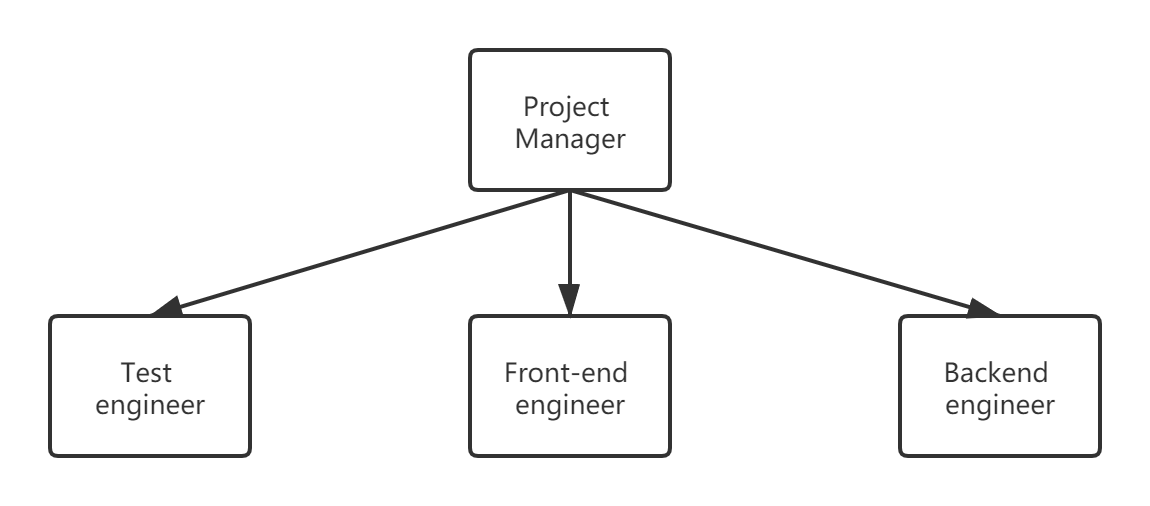
\includegraphics[width=4.5in]{figure/1.png}
\end{figure}
\textbf{Staffing management plan:}

\noindent
\textbf{Project Manager:} Project manager(PM) has the overall responsibility for the successful initiation, planning, design, execution, monitoring, controlling and closure of a project. PM plan and define scope of the project. manage the cost, time and resources of the project, and undertake the quality controlling responsibility.

\noindent\textbf{Test engineer:} Test engineers should write test plans, plan detailed test plans, and write test cases. In addition, the test engineer needs to put forward suggestions for further product improvement and evaluate whether the improvement plan is reasonable; summarize and statistically analyze the test results, track the test, and provide feedback.

\noindent\textbf{Front-end engineer:} The front-end engineer is responsible for the miniprogram development, he should develop adapt API from server side into client such as web browser and wechat miniprogram. 

\noindent\textbf{Backend engineer:} The back-end engineer is responsible for the server development. He should develop a robust and feasible server system. In this system, server structure includes mysql database, redis cache and django web application server.

\begin{table}
\centering
\begin{tabular}{|c|c|c|c|c|}
\hline
\multicolumn{5}{|c|}{\textbf{Responsibility assignment matrixes}}\\ % 用\multicolumn{3}表示横向合并三列 
                        % |c|表示居中并且单元格两侧添加竖线 最后是文本
\hline
\textbf{Task}&\textbf{Project Manager}&\textbf{Test engineer}&\textbf{Front-end engineer}&\textbf{Backend engineer}\\
\hline
Demand Analysis&P,R&P&P&P\\
\hline
Prototype Design&P,R&P&P&P\\
\hline
UI Design&P&P&P,R&P\\
\hline
Backend Development&N&N&N&P,R\\
\hline
Unit Test&N&R,P&N&N\\
\hline
Frontend Development&N&N&P,R&N\\
\hline
API Adaptation&N&N&N&P,R\\
\hline
App Deployment&N&N&N&P,R\\
\hline
Stress Test&N&P,R&N&N\\
\hline
Integration Testing&N&P,R&N&N\\
\hline
Code Review&N&P&P&P,R\\
\hline

\end{tabular}
\caption{R:Responsibility  N:None  P:Participate}
\end{table}

\section{Project execution}
%Each team should provide sufficient details about how the project is executed. Thus, using the milestones you have identified in your project plan, you are required to demonstrate how your team has executed the project. For each milestone, you should update your project progress in terms of schedule and cost. For each milestone, appropriate project progress reports need to be generated and you should use Microsoft Project to track your project progress (appropriate baseline should be used to track the project progress). In addition to the outputs from Microsoft Project, you may also want to include the following in the report: project staff assignment, change requests, project management plan updates, deliverables, and at least 4 meeting minutes in the report.

There are 3 phase in out project: Product Design, Development and Release. Accordingly, There is one according milestone in the end of each phase: Design Phase Finished, Development Finished and  Released.

\begin{figure}[H]
  \centering
  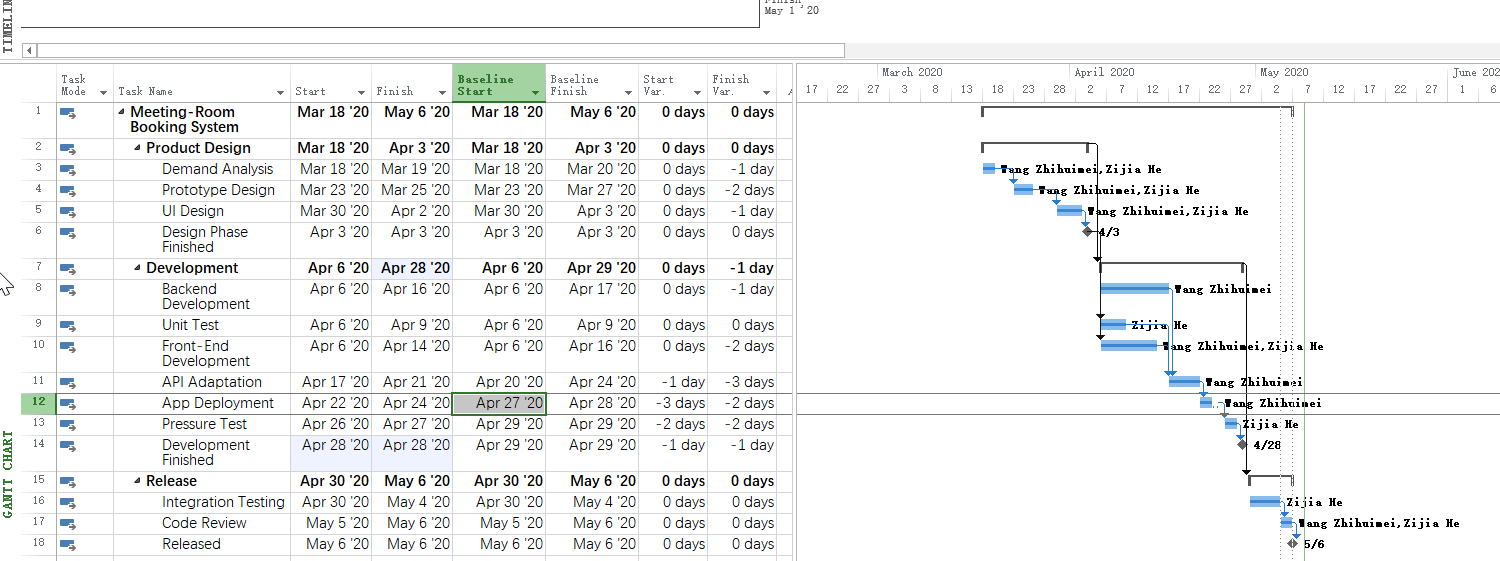
\includegraphics[width=1.0\textwidth]{figure/bls1}
  \caption{Difference between baseline and actual schedule}
  \end{figure}

\begin{figure}[H]
  \centering
  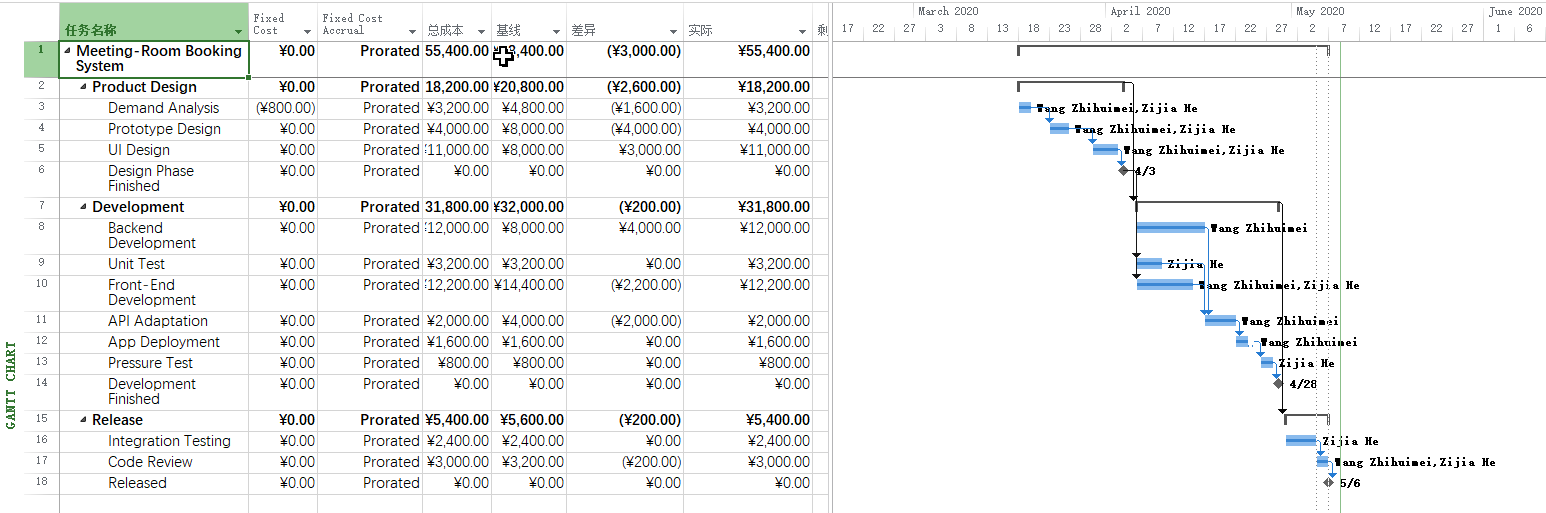
\includegraphics[width=1.0\textwidth]{figure/bls2}
  \caption{Difference between baseline and actual cost}
\end{figure}
  
\begin{figure}[H]
  \centering
  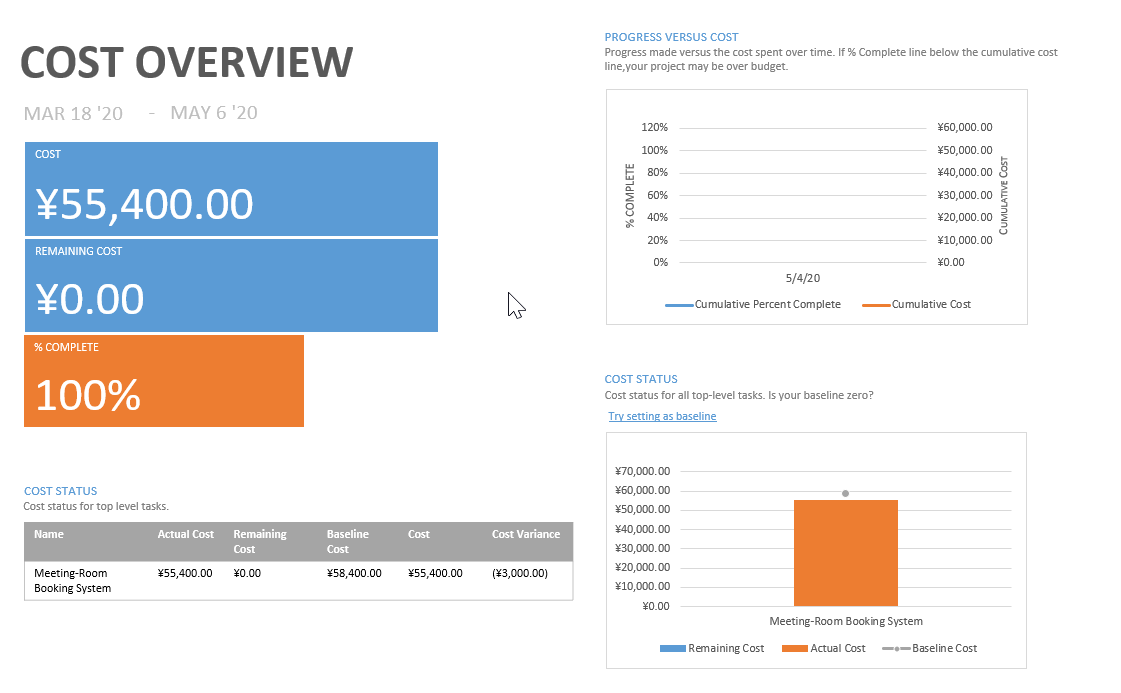
\includegraphics[width=1.0\textwidth]{figure/costrp}
  \caption{Cost report}
\end{figure}



\subsection{Product Design}
The baseline total cost is ¥20800, while the actual cost is ¥18200. 

\noindent This phase, our team performed Demand Analysis from Mar. 18 to Mar. 19 with the cost of ¥4800 and we finished this phase 1 day in advance compared with baseline. For the prototype design phase, we completed it two days in advance. The actual cost is ¥4000, only 50\% of the baseline cost. We completed the UI design phase 1 days in advance as well. We spend ¥3000 more than baseline ¥11000.

\begin{figure}[H]
  \centering
  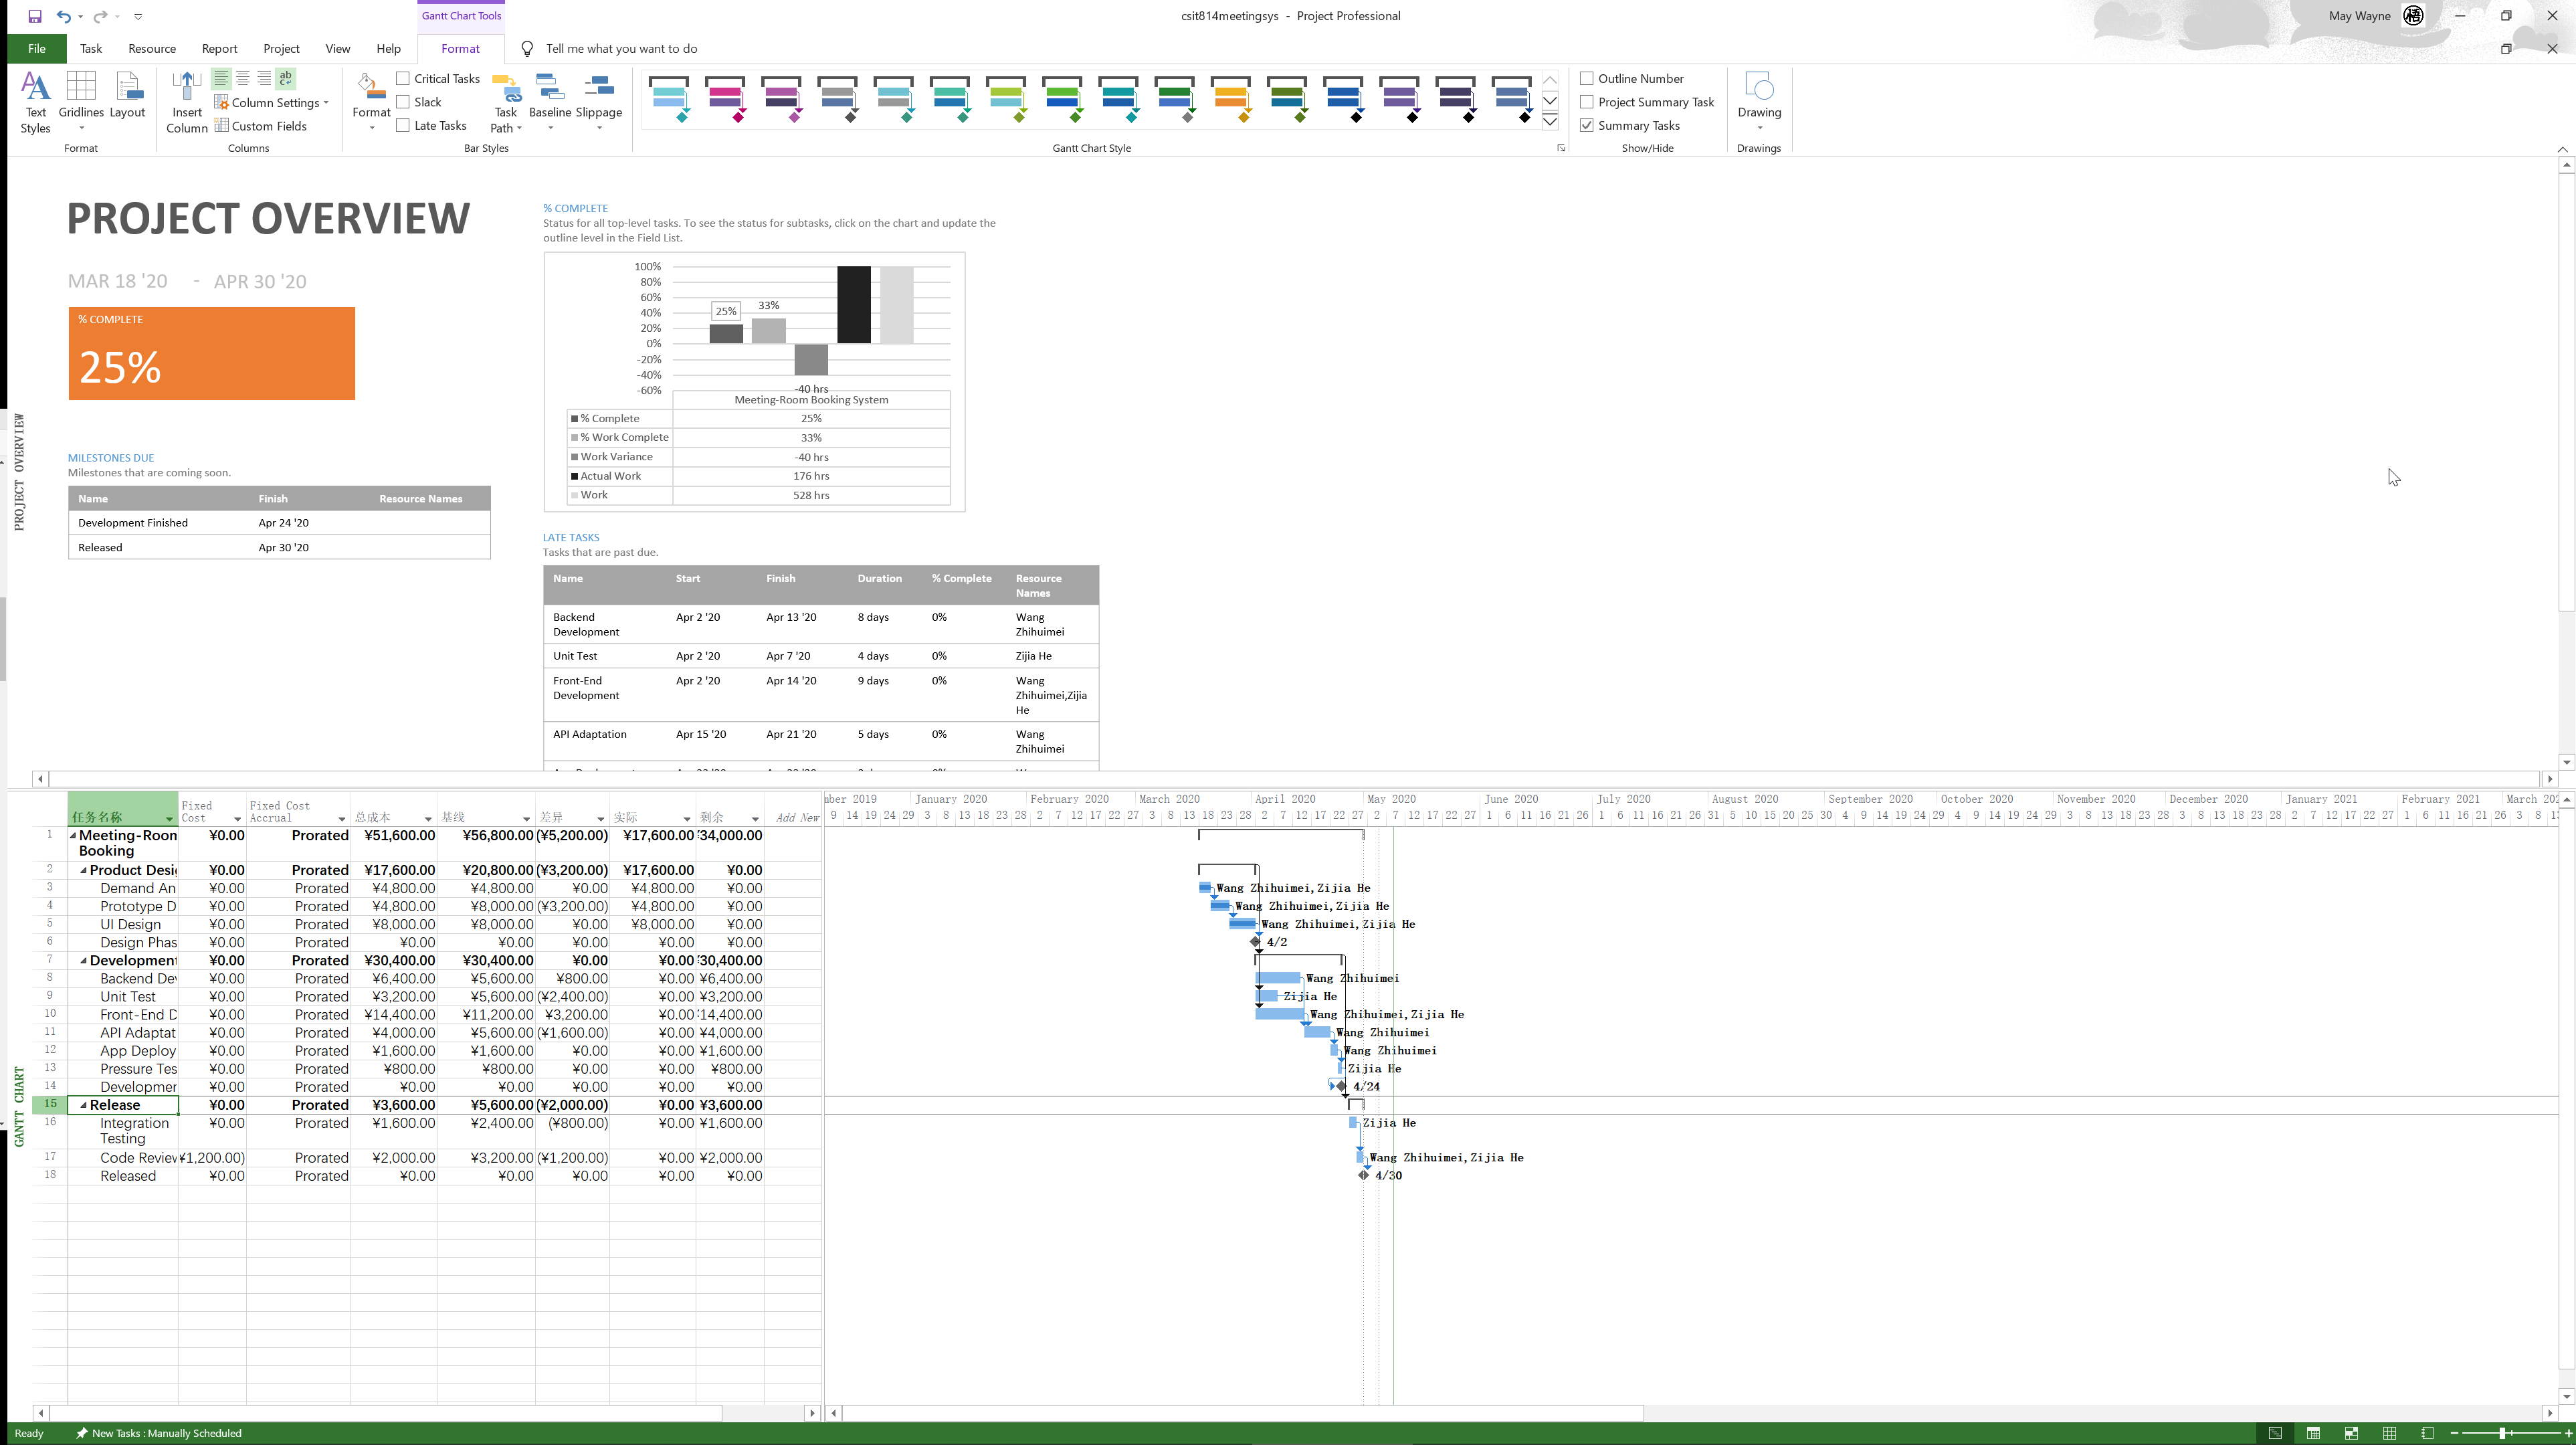
\includegraphics[width=1.0\textwidth]{figure/projrep1}
  \caption{Product Design Milestone Project report}
\end{figure}

\subsection{Development}
In this stage, the total baseline cost is ¥30400, while our team spend ¥32000 in this phase. The over-budget and delay happened mainly happened in back-end development and front-end development. The reason for this is that the difficulty of the development is underestimated. Besides, The demand change needs additional time to reassemble the modules and features of the system. But we accelerate the progress of other tasks, and we reach the milestone of this phase in advance by one day.

\begin{figure}[H]
  \centering
  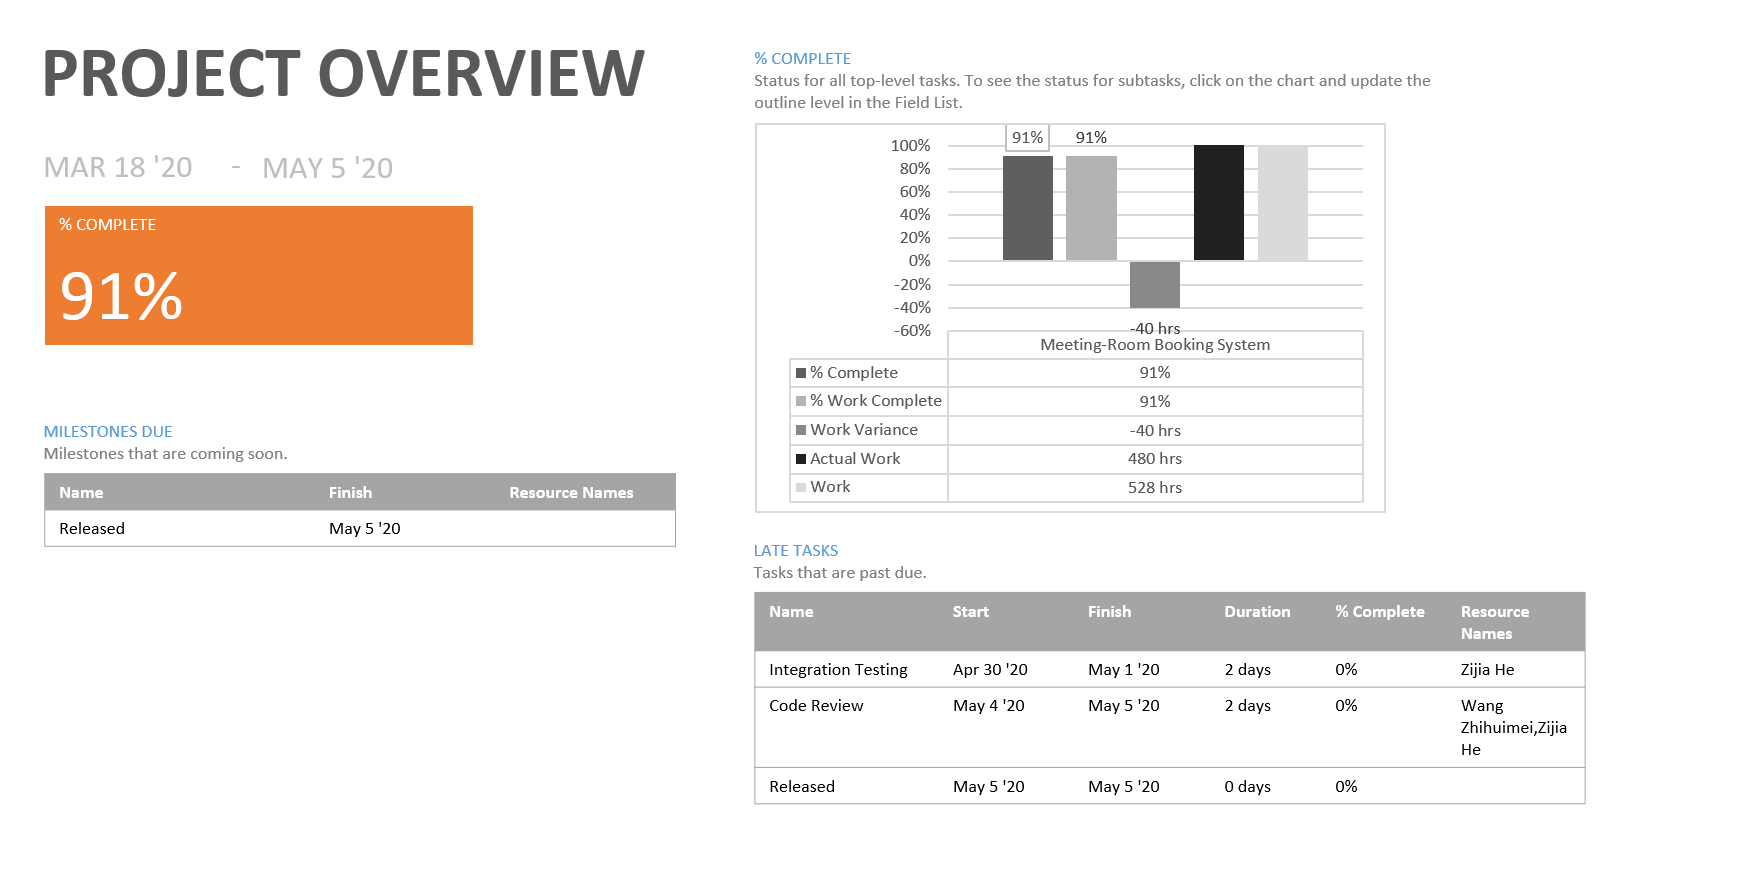
\includegraphics[width=1.0\textwidth]{figure/projrep2}
  \caption{Development Milestone Project report}
\end{figure}

\subsection{Release}
The total baseline cost is ¥5600, while the actual price is ¥4400, including ¥2400 in Integration test and ¥2000 in Code review, which is because we applied an automated test in testing tasks, which reduce the cost and accelerate the work progress. Finally, the milestone of Release "Released" come in advance for one day.

\begin{figure}[H]
  \centering
  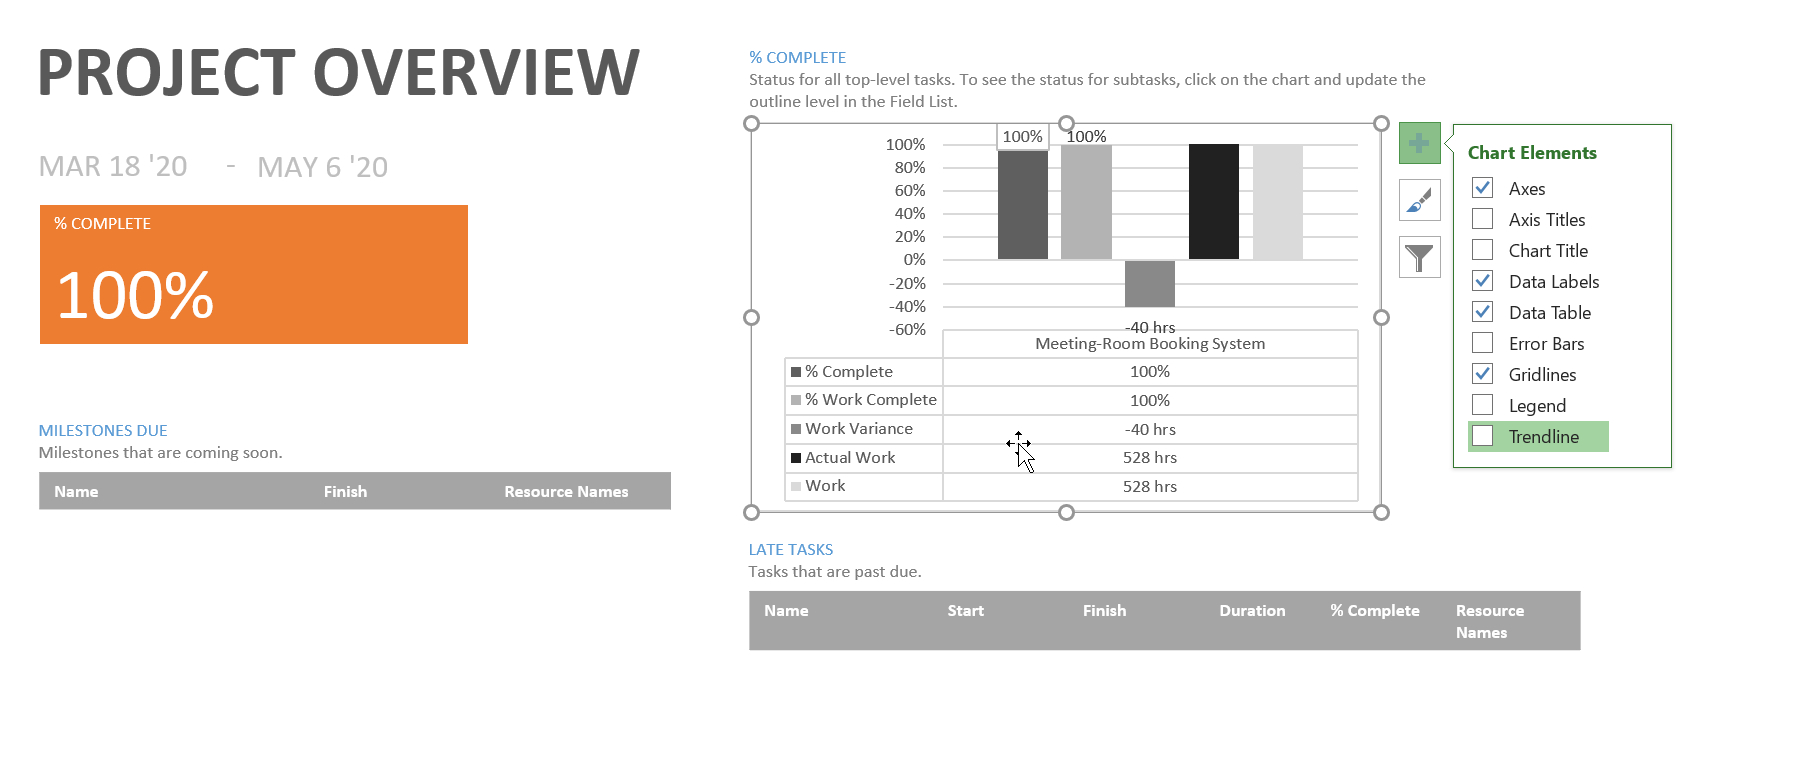
\includegraphics[width=1.0\textwidth]{figure/projrep}
  \caption{Release Milestone Project report}
\end{figure}


%TODO: milestone report%





\section{Project closing and Lessons-learnt}

%This part of the report should evaluate your project success against your initial plan. It should also answer questions like “Did the project meet scope, time, and cost goals?”, “What went right and what went wrong on this project?”, “What will you do differently on the next project based on your experience working on this project?”. You can refer to Table 3-16 (p.116 in your textbook) for a sample lessons-learnt report. %
\subsection{Did the project meet scope, time and cost goals}
Generally, Our system is consistent with the initial plan. We did the demand analysis and verified the real need of the user. We list must-to-have components and better-to-have components and build the prototype product. We have implemented the meeting booking system with server-side and client-side. We have deployed it in the WeChat mini-program, web browser and Linux server. The procedure runs typically with expected features implemented. But the performance of the system is limited as we use raspberry as a server, which can optimise by migrating the server side to a high-performance server.

\subsection{What went right and what went wrong on this project}
In general, the project meet the expected requirement. We deployed the system server-side in a Linux server, and release the WeChat mini program client publicly. User can use their WeChat account to register the system and can book a meeting room with a complete view of schedule and detail. The demand is satisfied generally.

We completed the project in advance, while some tasks (server-side and front-end development) exceed the deadline of the baseline. The baseline budget has some surplus as we spend RMB 51600 rather than expected RMB 56800. We have done a great job of controlling costs.

Also, the server-side development encountered some difficulties, such as database corrupt and redis cache system crashing. This is mainly because the development specifications are not strictly followed, with formal unit testing applied to the development, this problem is solved.




\subsection{What will we do differently on the next project}
\begin{itemize}
  \item Start small, then extend. Creating a mini prototype at first and then extend the solution step by step, until it does what it is supposed to. As no one is able to plan everything out in detail from the beginning.
  \item Change one thing at a time. When developing and something fail, or feature stops working. It's better to find the problem if only one thing of the system is changed.
  \item Add logging and error handling early. The logging system can be very helpful in the debugging and diagnosing procedure. It is a way of verifying how things going on in the system.  
  \item All new lines must be executed at least once. A new feature need immediate test to avoid spending time on debugging. Often, the best way is by automatic tests, but not always. But no matter what, every new line of code has to be executed at least once.
  \item Test the parts before the whole. Testing is a method to save time when developing new features. Often there are problems with integrating different parts. If you can trust that the parts work as expected, it becomes much easier to track down the integration problems.
  \item First understand the existing code. Most coding requires changing existing code in some way. Even if it is a new feature, it needs to fit into the existing program. And before you can fit the new stuff in, you need to understand the current solution. Otherwise you may accidentally break some of the existing functionality. This is means that reading code is a skill that is as necessary as writing code. It is also part of the reason why seemingly small changes can still take a long time – you must understand the context in which you make the change.
  \item Read and run. Understand and then develop. You can read the code, and you can run the code. Running the code can be a great help when figuring out what it does. Be sure to make use of both methods.
  \item Fix the known errors, then see what’s left. Sometimes there are several problems present that you know about. The different bugs can interact with each other and cause strange things to happen. Instead of trying to work out what happens in those cases, fix all the know problems and then see what symptoms remain.
  \item Correlate with timestamps. When troubleshooting, use the timestamp of events as a help. Look for even increments. For example, if the system restarted, and a request was sent out around 3000 milliseconds before, maybe a timer triggered the action that lead to the restart.
  \item Ask. Reading and running the code is often great for figuring out what it does and how it works. But if you have the possibility to ask someone knowledgeable (perhaps the original author), use that option too. Being able to ask specific questions, and follow-up questions to those, can give you information in minutes that would otherwise take days to get.
\end{itemize}

\end{document}

